\documentclass[a4paper,oneside]{article}
\usepackage[english,magyar]{babel}
\selectlanguage{magyar}

\usepackage[utf8]{inputenc}
\usepackage{t1enc}
\usepackage{multirow}
%================================================================
% Undorító dolog bitmappelt (Type III) betűtípust nézni a PDF-ben
% képernyőn. Az alapértelmezett Computer Modern font LaTex-ben
% bitmappelt, ezért használjunk Times fontot:
\usepackage{times}

\usepackage{graphicx}
\graphicspath{{./figs/}}

%================================================================
% Kötelezően használjuk a hyperref csomagot, mert ezzel többek között 
%  kultúrált hyperlinkelt PDF-et lehet csinálni az alábbi
%  variációkban, különféle hyperref backend-ekkel:
%  pdflatex,dvipdfm,ps2pdf
% tapsztalataim szerint a MikTeX (Win32) a 'dvipdfm' konverzióval
% optimális  míg a teTeX (Linux/Solaris) jobb szereti a 'dvips' módszert
%------------------------------------
% pontosan egyet kommentezzünk be!!!!!!!
% értelemszerűen backend függően generáljunk dvi-ból PDF-et!!!
%------------------------------------
% A hyperref csomag az utolsó beolvasott csomag legyen, kivéve néhány
% problémás csomagot, pl. algorithm
%-----------
% ########################### FONTOS ###########################
% A hyperref hibásan működik a babel csomag 'magyar.ldf' fájljának
% 1.5-ös verziójánál korábbi változatával. 2004. februárjában a MikTeX
% és teTex disztribúciók még csak a v.1.4 verziót tartalmazták! A fájl
% aktuális verziója a BME Matematikai intézet LaTeX honlapjáról
% elérhető: http://www.math.bme.hu/latex/ 
% A lusták kedvéért a jelen sablon mellé is mellékelem:
% magyarlatex_0.01-2.tar.gz 
% ########################### FONTOS ###########################
%-----------
% Ha nem akarunk .ps-t csinálni, csak egylépésben PDF-et, és nem
% ragaszkodunk az .eps  formátumú ábráinkhoz, akkor konvertáljuk az
% ábráinkat .pdf-be (epstopdf):  .tex --pdflatex-->  .pdf
%\usepackage[pdflatex]{hyperref}
% ----------
% Ha nem akarunk .ps-t csinálni, csak PDF-et, de ragaszkodunk az .eps
% formátumú ábráinkhoz: .tex --latex--> .dvi --dvipdfm--> .pdf
%\usepackage[dvipdfm]{hyperref} 
% ----------
% Ha  akarunk .ps-t is csinálni, meg  PDF-et is, és ragaszkodunk az .eps
% formátumú ábráinkhoz, 
% .tex --latex--> .dvi --'dvips -t a4'--> .ps --ps2pdf--> .pdf 
%\usepackage[ps2pdf]{hyperref}
%\usepackage[dvipdfm]{hyperref}
\usepackage[hidelinks]{hyperref}
\hypersetup{
    colorlinks=false,       % false: boxed links; true: colored links
    linkcolor=red,          % color of internal links
    citecolor=green,        % color of links to bibliography
    filecolor=magenta,      % color of file links
    urlcolor=black           % color of external links
}
\usepackage{tikz}
\usepackage{tkz-graph}
\usetikzlibrary{arrows,calc,automata,chains,matrix,positioning,scopes,decorations.pathmorphing,decorations.pathreplacing}
\usepackage{paralist}
\usepackage{epstopdf}

\usepackage[backend=bibtex,maxnames=6]{biblatex}
\addbibresource{refs.bib}

\usepackage{indentfirst}
\usepackage{setspace}
\usepackage{enumitem}
\usepackage{amsmath}
\usepackage{array}

\usepackage[format=hang]{caption}
\usepackage{subcaption}

%%%%%%%%%%%%%%%%%%%%%%%%%%%%%%%%%%%%%%%%%%%%%%%%%%%%%%%%%%%%%%%%%%
% Itt kezdődik a doksi maga
%%%%%%%%%%%%%%%%%%%%%%%%%%%%%%%%%%%%%%%%%%%%%%%%%%%%%%%%%%%%%%%%%%
\begin{document}

\onehalfspacing
\frenchspacing

%%%%%%%%%%%%%%%%%%%%%%%%%%%%%%%%%%%%%%%%%%%%%%%%%%%%%%%%%%%%%%%%%%%
% Ezt ne piszkáld!!!!
%%%%%%%%%%%%%%%%%%%%%%%%%%%%%%%%%%%%%%%%%%%%%%%%%%%%%%%%%%%%%%%%%%%
\pagestyle{myheadings} % legyen fejléc 

\newcommand{\onlabcim}{
  \begin{center}
    \huge{\textbf{Önálló laboratórium beszámoló}}

    \small{Távközlési és Médiainformatikai Tanszék}
  \end{center}
} 

% Argumentumok: #1=Név, #2=Neptunkód, #3=szakirány, #4=email, #5 konzulens-1, #6 konzulens-1-email, #7 konzulens-2, #8 konzulens-2-email
\newcommand{\onlabszerzo}[6]{

\begin{center}
  \begin{tabular}{ p{3cm} p{7.5cm} }
  
  Készítette: & \textbf{Kriván Bálint}  \\
  Neptun-kód: & \textbf{CBVOEN}  \\
  Ágazat: & \textbf{#1}  \\
  E-mail cím: & \href{mailto:#2}{\textbf{#2}}  \\
  Konzulens: & \textbf{#3}  \\
  E-mail cím: & \textbf{#4} \\
  
  \end{tabular}
\end{center}

}

% % Argumentumok: #1=Név, #2=email
% \newcommand{\konzulens}[2]{
%   \noindent\textbf{Konzulens:} #1 
%   \newline\emph{Email cím:}\/ \href{mailto:#2}{#2}
%   \newline
% 
% }

% Argumentumok: #1=Tanév (xxxx/xx alakban, #2=félév (pont nélkül)
\newcommand{\tanevfelev}[2]{
  \large\noindent\textbf{Tanév:} #1. tanév, #2. félév
  \newline
}

% Argumentumok: #1=téma címe 
\newcommand{\feladatcim}[1]{
  \large\noindent\textbf{Téma címe: #1}
  \bigskip
}

% Argumentumok: #1=téma részletei 
\newcommand{\feladatmaga}[1]{
\large\noindent\textbf{Feladat:} 
  \newline
 #1
 \newline
 \smallskip
}

% A fejezetek közé beágyazott irod.jegyzék
\def\thebibliography#1{\renewcommand{%
\baselinestretch}{1}\subsection{A tanulm\'anyozott irodalom jegyz\'eke}\list
 {\small [\arabic{enumi}]}{\settowidth\labelwidth{[#1]}\leftmargin\labelwidth
 \advance\leftmargin\labelsep
 \usecounter{enumi}}
 \def\newblock{\small \hskip .11em plus .33em minus .07em}
 \sloppy\clubpenalty4000\widowpenalty4000
 \sfcode`\.=1000\relax}
\let\endthebibliography=\endlist%


%%% Local Variables: 
%%% mode: latex
%%% TeX-master: "template"
%%% End: 


\markright{Kriván Bálint (CBVOEN)} % egyoldalas fejléc!!!
%--------------------------------------------------------------------
% fedlap
%--------------------------------------------------------------------
\begin{titlepage}
%bme logo 
 \begin{figure}[h]
    \centering
      
\includegraphics[width=12cm]{bme_logo.eps}
  \label{fig:bme_logo}
  \end{figure}
  % nincs fejléc a címlapon!!
  \thispagestyle{empty}
  %cím generálás
  \onlabcim

  \onlabszerzo{Hálózatok és szolgáltatások}{balint@krivan.hu}{Kovács Gábor}{kovacsg@tmit.bme.hu}
  
  \feladatcim{Videofelvételek 3D rekonstrukciója és transzformációja}

  \feladatmaga{XXX}
  
  \tanevfelev{2013/14}{2}
 
\end{titlepage} 

%==================================================================
\section{A laboratóriumi munka környezetének ismertetése, a munka előzményei és kiindulási állapota}
\label{sec:bevezeto}

\subsection{Bevezetés/elméleti összefoglaló}
\label{sec:bevez-ossz}

\textit{Ide jön valami, ha kiderül, hogy kell még hely. Illetve le lehet írni, hogy az előző félévben csináltak itt is jók stb.}

\subsection{A munka állapota, készültségi foka a félév elején}
\label{sec:munka-allap-kesz}

Az előző félév során az Önálló laboratórium 1 című tárgy keretében megismerkedtem az OpenCV keretrendszerrel, valamint az általa használt kameramodellel és egy lézerpont detektálásának lehetőségeit jártam körben. A jelenlegi félévben így nem kellett elölről kezdeni mindent, ott folytathattam ahol abbahagytam. A jelenlegi félév fő célja, hogy videofelvételeket -- azon belül egy képkockát -- tudjunk rekonstruálni 3D-ben.

\newpage
%==================================================================
\section{Az elvégzett munka és az eredmények ismertetése}
\label{sec:az-elvegzett-munka}

\subsection{Sztereó-kalibráció}
\label{sec:sztereo-kalibracio}

Az előző félévben még csak egy kamerát használtam, de a 3D rekonstrukcióhoz szükség van sztereókamerák alkalmazására. A félév során két darab azonos gyártmányú webkamerát vettem igénybe. Mielőtt az általuk készített képeket használni tudnánk szükséges egy kalibráció.

A kalibráció során két lényegében eltérő paraméterhalmazt nyerhetünk ki. Az egyik a kamerák tulajdonságaiból adódnak (fókusz-távolság, torzítási paraméterek), ahogy azt az előző félévben is láttuk. A második pedig a két kamera egymáshoz viszonyított helyzete (eltolás, forgatás). A kalibráció során megkaphatjuk azokat a transzformációkat is (a torzítás helyreállítása mellett), melyek a két kamera képét úgy transzformálják, hogy az azonos pontok egy egyenesbe essenek. Felhasználva, hogy az egymásnak megfelelő képpontok csak $x$ irányban térnek el, a két képből a 3D-s pontfelhő helyreállításának számítási komplexitása egyszerűsödik.

Hasonlóan az előző félévhez, most is egy sakktábla mintát fogunk használni a kalibrációhoz. A sakktáblát különböző pozícióban a két kamera által készített képen detektáljuk, majd a mezők sarkainak pozíciói alapján kiszámoljuk az előzőekben említett paramétereket, melyekhez az OpenCV rendelkezésre bocsájt különböző függvényeket.

\begin{figure}[tbh]
  \centering
  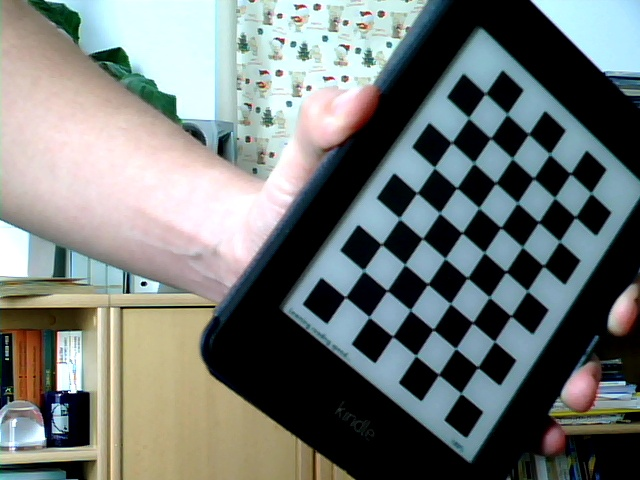
\includegraphics[width=160pt]{figs/left07.jpg}\hspace{10pt}
  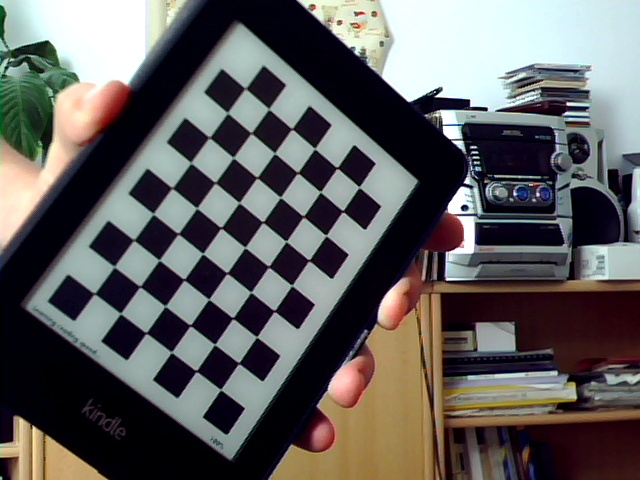
\includegraphics[width=160pt]{figs/right07.jpg}
  \caption{A kalibrációhoz felhasznált egyik képpár \label{fig:imagepairs}}
\end{figure}

\begin{figure}[tbh]
  \centering
  \begin{tikzpicture}[x=330,y=330]
	\node[anchor=south west,inner sep=0] at (0.515151,0) {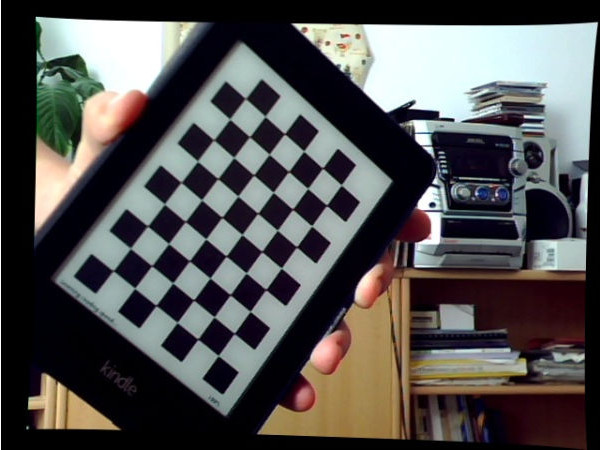
\includegraphics[width=160pt] {figs/calibrated_right.jpg}};
    \node[anchor=south west,inner sep=0] at (0,0) {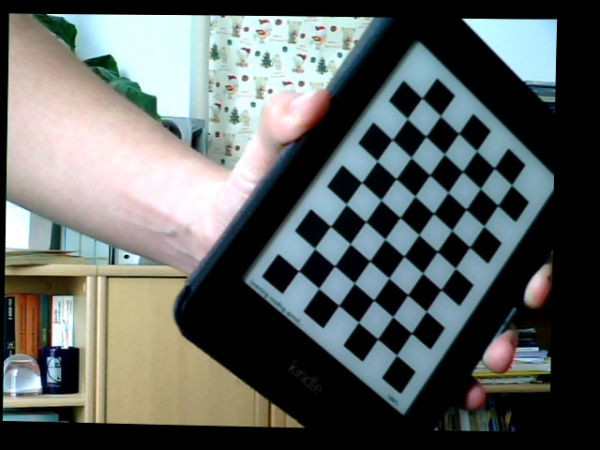
\includegraphics[width=160pt]    {figs/calibrated_left.jpg}};
    \draw[red,thick] (0,0.301) -- (1,0.301);
    \draw[red,thick] (0,0.200) -- (1,0.200);
    \draw[red,thick] (0,0.140) -- (1,0.140);
    \draw[red,thick] (0,0.045) -- (1,0.045);
\end{tikzpicture}
  \caption{Kalibráció után az előző képpár \label{fig:calibrated}}
\end{figure}

A példák között található egy minta-alkalmazás, ami két rögzített kamera bal- és jobbkép listája alapján kalibrál. Ezt átalakítottam és két részre bontottam. Készült egy egyszerű alkalmazás, ami a két USB-n csatlakoztatott kamera képeit könnyen elmenthetjük fájlokba (\texttt{leftxx.jpg} és \texttt{rightxx.jpg} lásd \aref{fig:imagepairs}. ábra), valamint egy másik, ami ezeket megtalálva elkészíti a kalibrációs fájlokat, melyeket a tényleges alkalmazásunk felolvashat. Ez azért fontos, mert így a tényleges kalibráció a feladat többi részétől elkülöníthető és egy statikus térrészről több pozícióban is készíthetünk ugyanazon kamerákkal képeket. \Aref{fig:calibrated}. ábrán látható, hogy a képpontok valóban egy egyenesbe esnek (balfelső és a jobbalsó sarokban állított egyenesek), valamint, hogy ha relatíve jól pozicionáljuk a kamerákat akkor a transzformáció után a kapott képek legnagyobb része hasznos információt tartalmaz.

\subsection{3D-rekonstrukció}

\begin{figure}[tbh]
  \centering
\definecolor{ffqqqq}{rgb}{1.0,0.0,0.0}
\definecolor{qqqqff}{rgb}{0.0,0.0,1.0}
\begin{tikzpicture}[line cap=round,line join=round,>=triangle 45,x=1.0cm,y=1.0cm]
\clip(-1.5,-1.15) rectangle (4,7);
\draw [dotted,domain=-5.700000000000001:0.5] plot(\x,{(-0.0--0.75*\x)/-0.5});
\draw [dotted,domain=1.98:15.480000000000002] plot(\x,{(-1.875--0.75*\x)/0.52});
\draw [dotted,domain=0.5:15.480000000000002] plot(\x,{(-0.75--0.75*\x)/0.5});
\draw [dotted,domain=-5.700000000000001:1.98] plot(\x,{(-1.125--0.75*\x)/-0.48});
\draw [color=qqqqff,domain=0.5:15.480000000000002] plot(\x,{(-3.9375--6.75*\x)/0.75});
\draw [color=ffqqqq,domain=0.5:15.480000000000002] plot(\x,{(-1.9375--2.75*\x)/0.75});
\draw [color=ffqqqq,domain=-5.700000000000001:1.98] plot(\x,{(-4.8975--2.75*\x)/-0.73});
\draw [color=qqqqff,domain=-5.700000000000001:1.98] plot(\x,{(-12.817499999999999--6.75*\x)/-0.73});
\draw (0.0,0.0)-- (1.0,0.0);
\draw (1.5,0.0)-- (2.5,0.0);
\draw (2.75,6.0)-- (3.75,6.0);
\draw (3.75,2.0)-- (2.75,2.0);
\begin{scriptsize}
%\draw [fill=qqqqff] (0.0,0.0) circle (1.5pt);
%\draw [fill=qqqqff] (1.5,0.0) circle (1.5pt);
\draw (0.5,-0.75) circle (1.5pt);
\draw[color=qqqqff] (0.5,-1.02) node {$C1$};
\draw (1.98,-0.75) circle (1.5pt);
\draw[color=qqqqff] (2.1,-1.06) node {$C2$};
\draw [fill=ffqqqq] (1.25,2.0) circle (1.5pt);
\draw [fill=qqqqff] (1.25,6.0) circle (1.5pt);
\draw [fill=ffqqqq] (1.780909090909091,-0.0) circle (1.5pt);
\draw [fill=ffqqqq] (0.7045454545454546,-0.0) circle (1.5pt);
\draw [fill=qqqqff] (0.5833333333333334,-0.0) circle (1.5pt);
\draw [fill=qqqqff] (1.8988888888888888,-0.0) circle (1.5pt);
\draw [fill=qqqqff] (3.3333333333333335,6.0) circle (1.5pt);
\draw [fill=qqqqff] (3.148888888888889,6.0) circle (1.5pt);
\draw [fill=ffqqqq] (3.030909090909091,2.0) circle (1.5pt);
\draw [fill=ffqqqq] (3.4545454545454546,2.0) circle (1.5pt);
\end{scriptsize}
\end{tikzpicture}
\caption{Mélység és a \textit{disparity map} kapcsolata \label{fig:depth}}
\end{figure}

Kalibráció után rendelkezésre áll minden információ, amire szükségünk lesz a 3D-s pontfelhő megalkotására. OpenCV-ben találhatunk egy \texttt{reprojectImageTo3D} \cite{opencv-reprojectImageTo3D} nevű függvényt, mely pontosan ezt csinálja, de ehhez szükségünk van egy \textit{disparity map}re. Ez azt írja le, hogy egy adott pont a két képen mekkora $\Delta x$ távolságra van egymástól. Könnyű meggondolni, hogy ha egy pont a kamerákhoz közel van akkor ez a távolság nagy, ha távol akkor pedig kicsi, lásd \aref{fig:depth}. ábra. Ennek felhasználásával adhatunk mindegyik képpontnak mélység információt, így nyerhetjük a 3D-s pontfelhőt.

A szakirodalomban sokféle algoritmust találhatunk \cite{disparity-pixel} \cite{disparity-belief} \cite{disparity-dense-from-sparse}, amellyel két képpár alapján kiszámolhatjuk a disparity mapet, ezek egymástól sebességben, valamint abban térnek el, hogy különféle típusú képekre jobb/pontosabb megoldást adnak. A fő probléma ezek megítélésénél, hogy főleg jól ismert -- úgymond ,,referencia'' -- képekre, szekvenciákra vannak tesztelve, optimalizálva és egymással összehasonlítva, nem pedig való életbeli képekkel, ami igencsak eltorzítja a valós gyakorlati példákon történő alkalmazásukat/alkalmazhatóságukat. Úgy döntöttem, hogy az egyszerűség kedvéért az OpenCV-ben implementált megoldások közül választom ki a legjobbnak tűnőt, és nem kezdek el megírni egyet valamelyik publikáció alapján. Természetesen későbbiekben ez az implementáció lecserélhető, ha a következő félévek során találunk olyan algoritmust, amit célszerűbb alkalmazni.

Az OpenCV három implementációt tartalmaz: \texttt{StereoBM}, \texttt{StereoSGBM} \cite{disparity-sgbm} és \texttt{StereoVar} \cite{disparity-var}. Ezeket kipróbálva arra jutottam, hogy számomra a \texttt{StereoSGBM} a megfelelő. \Aref{fig:disparities}. ábrán látható az algoritmusok által visszaadott eredmények vizuális megjelenítése (a világosabb szín közelebbi pontot jelent).

\begin{figure}[tbh]
  \centering
  \begin{subfigure}[b]{.5\linewidth}
	\centering
	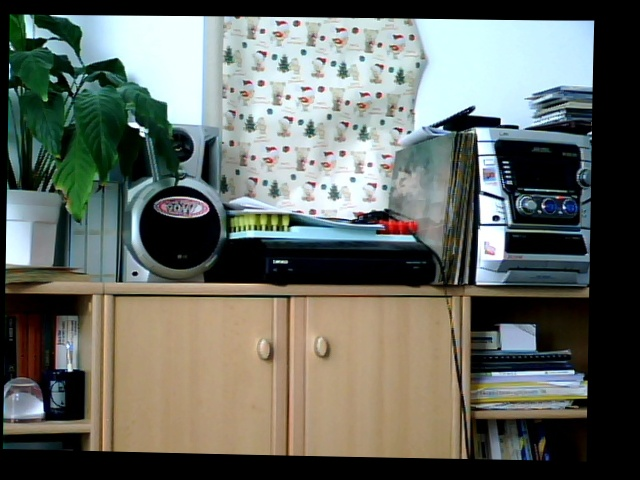
\includegraphics[width=160pt]{figs/left01_mapped.jpg}
	\caption{A rektifikált baloldali kép}
  \end{subfigure}%
  \begin{subfigure}[b]{.5\linewidth}
	\centering
    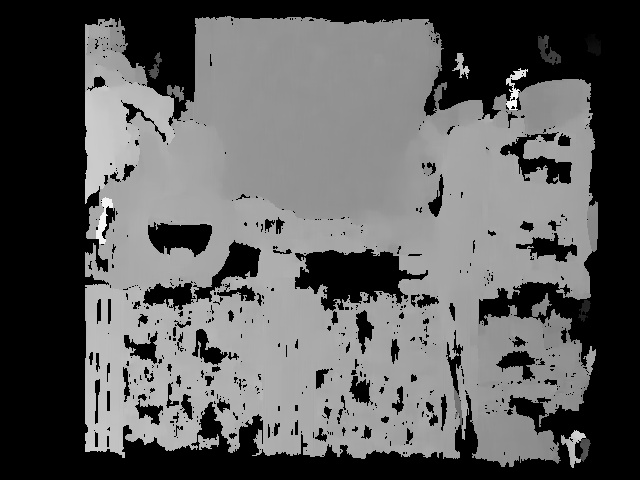
\includegraphics[width=160pt]{figs/disparity_bm.jpg}
	\caption{\texttt{StereoBM}}
  \end{subfigure}
  \begin{subfigure}[b]{.5\linewidth}
	\centering
	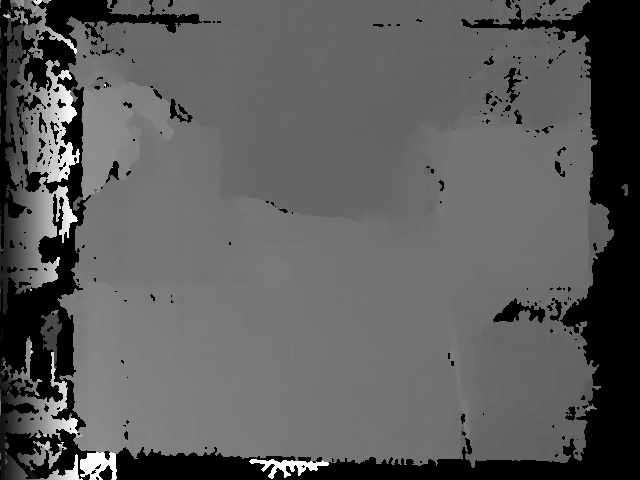
\includegraphics[width=160pt]{figs/disparity_sgbm.jpg}
	\caption{\texttt{StereoSGBM}}
  \end{subfigure}%
  \begin{subfigure}[b]{.5\linewidth}
	\centering
    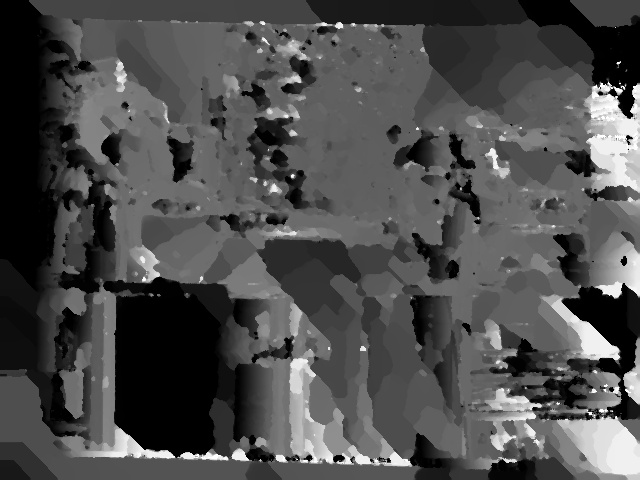
\includegraphics[width=160pt]{figs/disparity_var.jpg}
	\caption{\texttt{StereoVar}}
  \end{subfigure}
\caption{A baloldali kép és az algoritmusok által adott eredmények \label{fig:disparities}}
\end{figure}

Megfigyelhető, hogy a \texttt{StereoSGBM} adja a legjobb eredményt és szinte alig lassabb a \texttt{StereoBM}-nél. Bárhogy próbálkoztam, nem sikerült a \texttt{StereoVar}-t értékelhetően felparaméterezni, hogy használható eredményt adjon. A későbbiekhez még fontos, hogy csak a használható eltolás-értékeket vegyük figyelembe, jól látható, hogy a \texttt{StereoSGBM} a bal oldali részen ,,fura'' értékeket ad, ez annak köszönhető, hogy a világnak az a része a jobb oldali képen nem látható, így nem tudja ezt kiszámolni rendesen.

Miután megvan a disparity map, meghívhatjuk a \texttt{reprojectImageTo3D} függvényt a megfelelő argumentumokkal és megkaphatjuk a 3D pontfelhőt. Ezt könnyen megjeleníthetjük OpenGL segítségével, vagy kimenthetjük egy jól ismert szöveges formátumba, pl. PLY (Stanford Triangle Format) vagy PCD (Point Cloud Data). Ennek eredménye \aref{fig:pcd}. ábrán látható.

\begin{figure}[tbh]
  \centering
  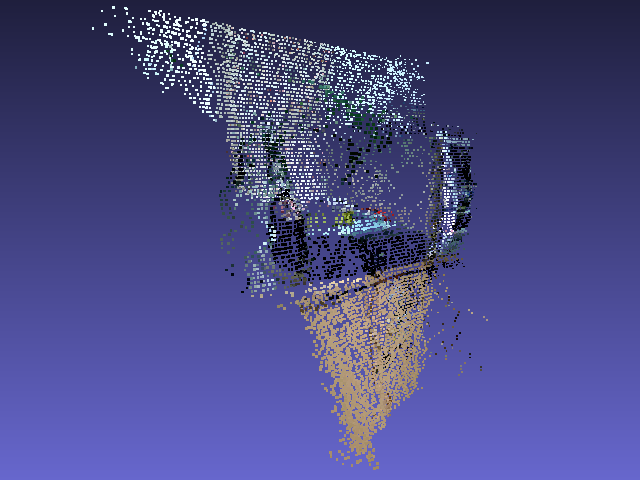
\includegraphics[width=100pt]{figs/snapshot00.png}
  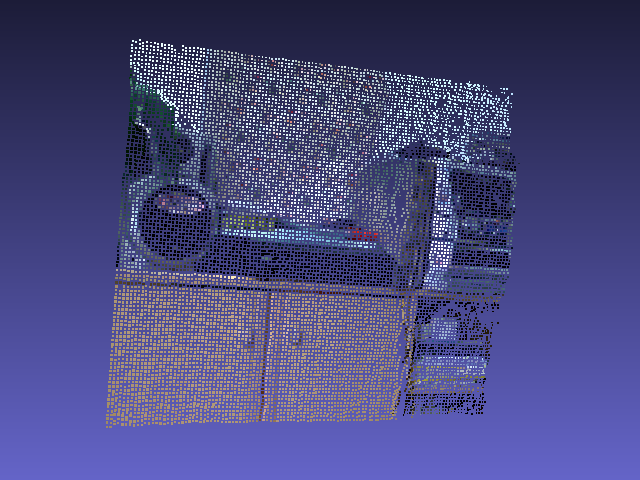
\includegraphics[width=100pt]{figs/snapshot01.png}
  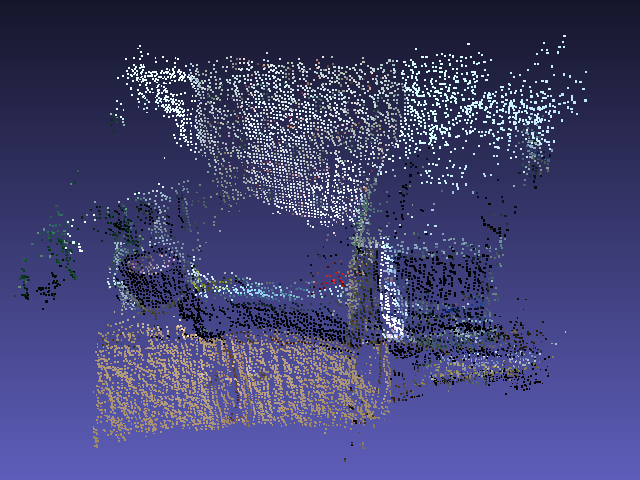
\includegraphics[width=100pt]{figs/snapshot02.png}
  \caption{A 3D-s pontfelhő megjelenítése balról, majdnem szemből és kissé felülről \label{fig:pcd}}
\end{figure}

Tekintve a webkamerák rossz minőségét egészen értékelhető eredményt kaptunk.

\subsection{Pontfelhő simítása, \textit{mesh} (objektum-háló) készítése}

Az előzőekben ismertetett eredményeknél nem álltam meg, megnéztem, hogyan lehet egy kicsit szebbé, és a későbbiekben használhatóbbá tenni az eredményt. Ha a pontfelhőből egy \textit{mesh}t tudnánk készíteni és azt a kamera által készített képpel textúrázni akkor sokkal szebb/simább eredményt kaphatunk.

Ehhez az OpenCV-n kívül egy másik ingyenesen elérhető és nyílt forráskódú alkalmazáskönyvtárat vettem igénybe, a PCL-t \cite{pcl}.

\subsubsection{Mesh számolás pontfelhőre}

Először nézzük meg, hogy a PCL-ben milyen beépített lehetőségeink vannak. Felületek számítására két alapvetően különböző módszercsalád közül választhatunk: az egyik a \texttt{MeshConstruction}, ahol a pontokat változatlanul hagyva próbáljuk őket összekötni és így egy hálót alkotni, a másik pedig a \texttt{SurfaceReconstruction}, ahol már a pontokat is módosítva alakítunk ki egy felületet. A következőkben az első családból nézünk meg 2 eljárást.

Tekintve, hogy a pontfelhőnk rendezett (azaz a vertexeket úgy kaptuk, hogy egy kép pixeleihez rendeltünk mélységet), használhatjuk az \texttt{OrganizedFastMesh} \cite{organizedfastmesh} algoritmust, ami a rendezettséget felhasználja a szomszédos pontok összekötéséhez. Egyetlen egy paraméterünk van, mégpedig a háromszögek éleinek hossza pixelben, minél nagyobbat választunk annál durvább lesz a felület, de így áthidalhatóak a nagyobb hézagok. \Aref{fig:fastmesh}. ábrán láthatunk néhány felületet különböző paraméterekkel.

\begin{figure}[tbh]
  \centering
  \begin{subfigure}[b]{.24\linewidth}
	\centering
	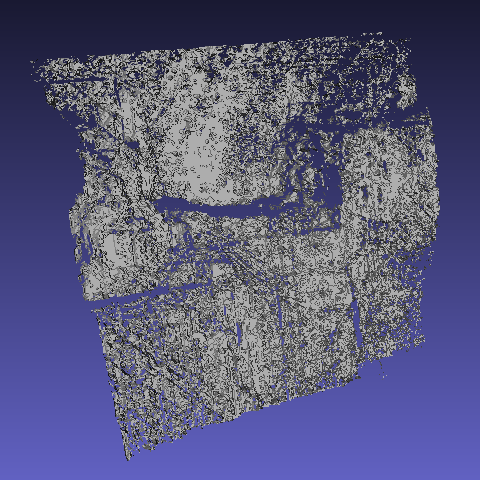
\includegraphics[width=75pt]{figs/fastmesh1.png}
	\caption{\label{fig:fastmesh1}}
  \end{subfigure}%
  \begin{subfigure}[b]{.24\linewidth}
	\centering
    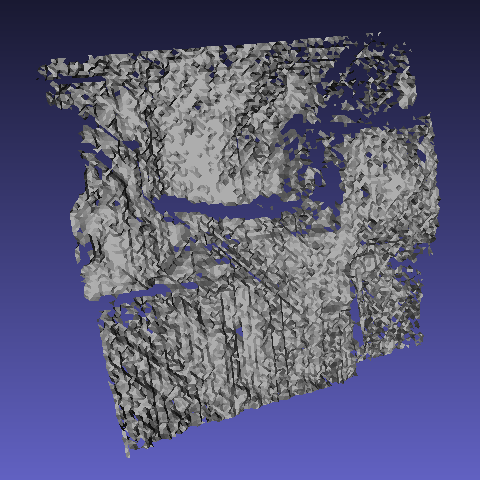
\includegraphics[width=75pt]{figs/fastmesh5.png}
	\caption{\label{fig:fastmesh5}}
  \end{subfigure}
  \begin{subfigure}[b]{.24\linewidth}
	\centering
	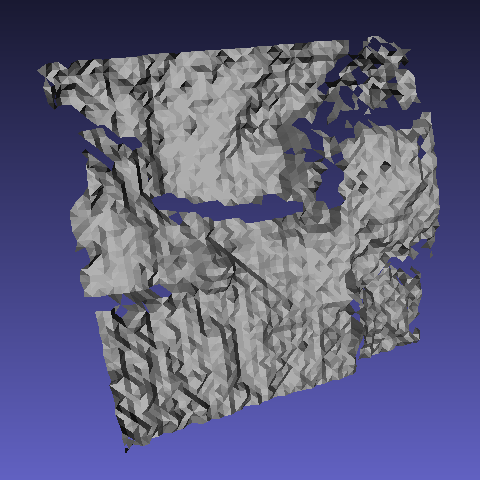
\includegraphics[width=75pt]{figs/fastmesh9.png}
	\caption{\label{fig:fastmesh9}}
  \end{subfigure}%
  \begin{subfigure}[b]{.24\linewidth}
	\centering
    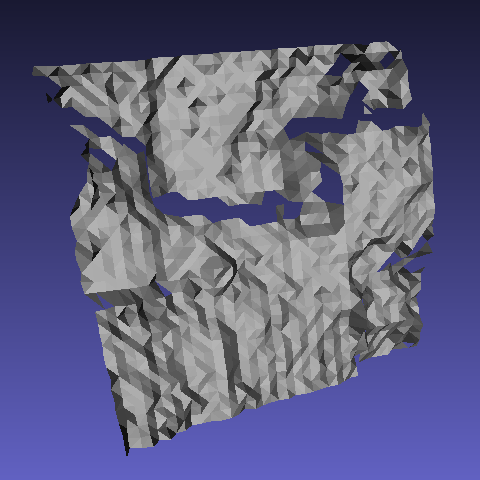
\includegraphics[width=75pt]{figs/fastmesh13.png}
	\caption{\label{fig:fastmesh13}}
  \end{subfigure}
\caption{\textit{a)} 1, \textit{b)} 5, \textit{c)} 9 valamint \textit{d)} 13 pixel hosszú háromszögoldalak \label{fig:fastmesh}}
\end{figure}

Textúrázhatóság szempontjából 9-től felfelé értékelhető, de jól látszódik, hogy az eredeti pontfelhő ,,rusztikusságából'' adódóan az így kapott felület is az, hiszen a vertexek pozícióján nem változtatunk, csak összekötjük őket.

A másik megvizsgált algoritmus a \texttt{GreedyProjectionTriangulation} \cite{greedy}. Lényege, hogy mohón (lokális szomszédsági viszonyokat vizsgálva) növeszti a háromszöghálót a beállított paramétereknek megfelelően, felhasználva a vertexek normáljait (melyeket megbecsülhetünk szintén lokális szomszédsági adatokat vizsgálva). Ennek több állítható paramétere van, amelyek közül a három legfontosabb: keresési sugár (lényegében egy felső korlát a háromszög oldalhosszaira), szomszédok száma (hány szomszédot vizsgáljon meg), valamint egy $\mu$ paraméter, ami azt szabályozza, hogy maximum hányszor messzebb lehet egy potenciális szomszéd a legközelebbi szomszédnál, hogy még összeköthetőnek minősítse. Néhány paraméterkombinációt megvizsgálva kapjuk \aref{fig:greedy}. ábrán látható hálókat.

\begin{figure}[tbh]
  \centering
  \begin{subfigure}[b]{.32\linewidth}
	\centering
	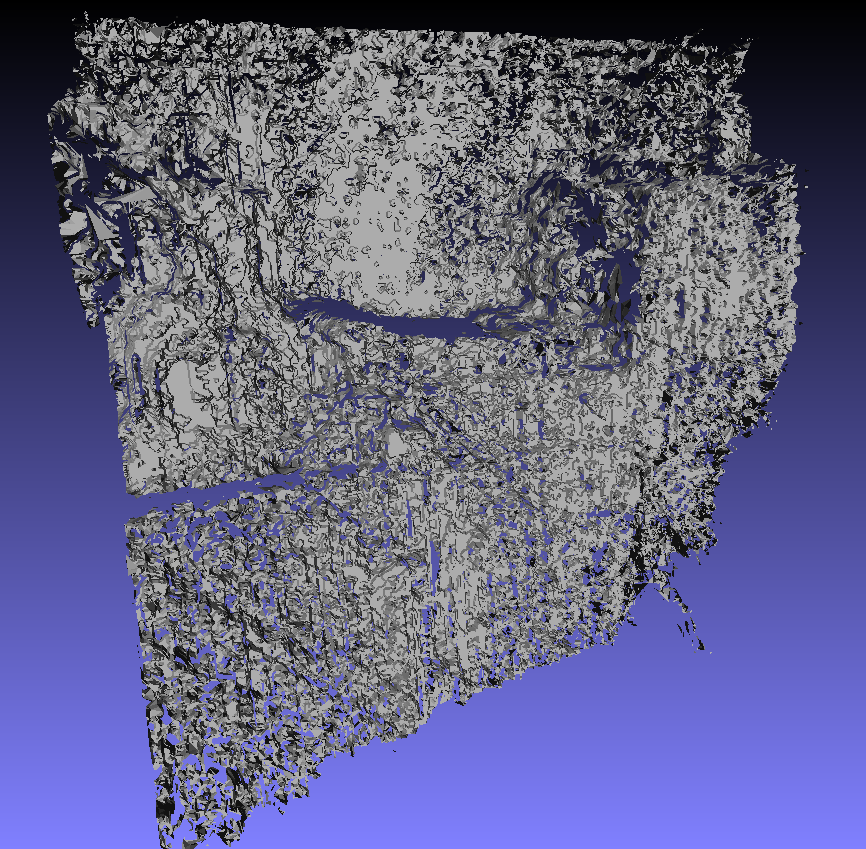
\includegraphics[width=100pt]{figs/greedy_50_2_5.png}
	\caption{\label{fig:greedy50}}
  \end{subfigure}%
  \begin{subfigure}[b]{.32\linewidth}
	\centering
	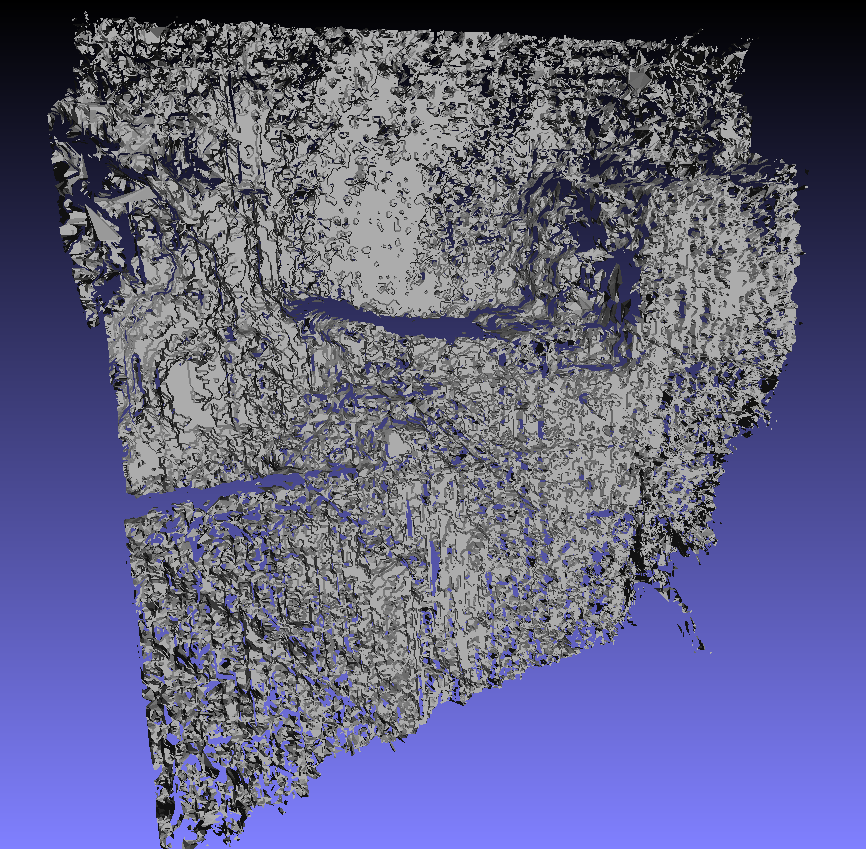
\includegraphics[width=100pt]{figs/greedy_100_2_5.png}
	\caption{\label{fig:greedy100_1}}
  \end{subfigure}%
  \begin{subfigure}[b]{.32\linewidth}
	\centering
	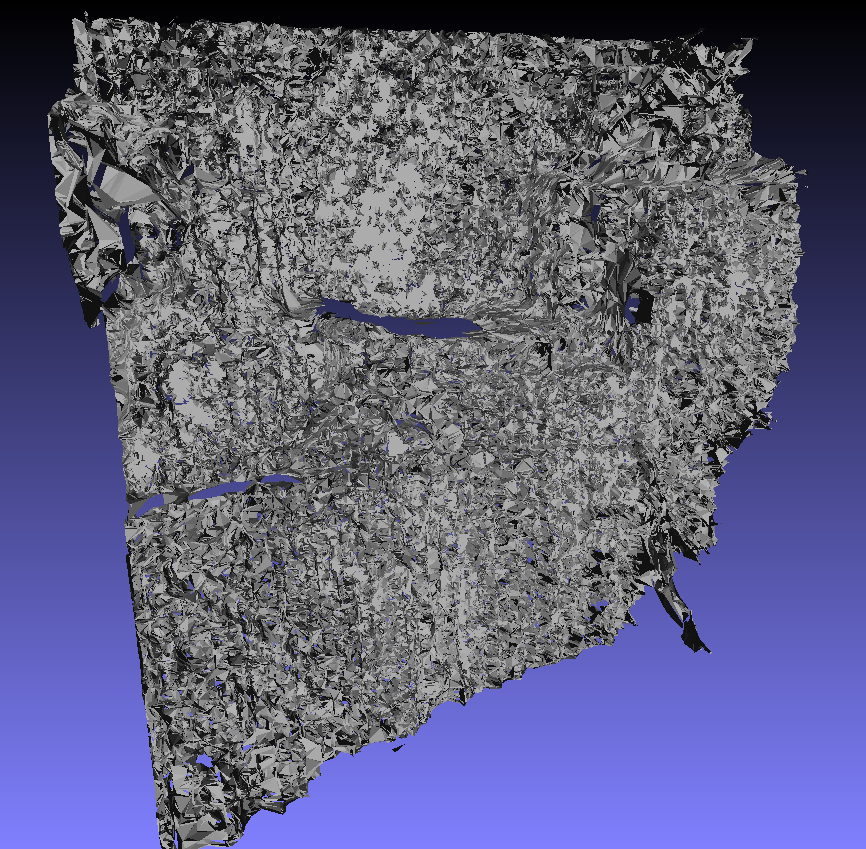
\includegraphics[width=100pt]{figs/greedy_100_10.png}
	\caption{\label{fig:greedy100_2}}
  \end{subfigure}%
\caption{50 és 100 szomszéd vizsgálata $\mu=2,5$-tel, valamint 100 szomszéd $\mu=10$-zel, a sugár fixen $1,5$ \label{fig:greedy}}
\end{figure}

A keresési sugár lényegében a sebességen változtat jelentősen, a háló mintájáért jelen esetünkben csak az volt a fontos, hogy az összekötendő pontok biztosan beleessenek az adott gömbbe. A szomszédok darabszáma jelentősen nem befolyásolja az összeköthetőséget, hiszen általában mindig van egy relatíve közeli pont, így a $\mu$ a domináns. Ha ezt növeljük, akkor távol eső pontok is összekötődnek, viszont a pontfelhő nem elég sima, így az elkészült felület (\ref{fig:greedy_closeup}. ábra) nagyon ,,meredek'', valamint az is látható, hogy továbbra is vannak hézagok.

\begin{figure}[tbh]
	\centering
	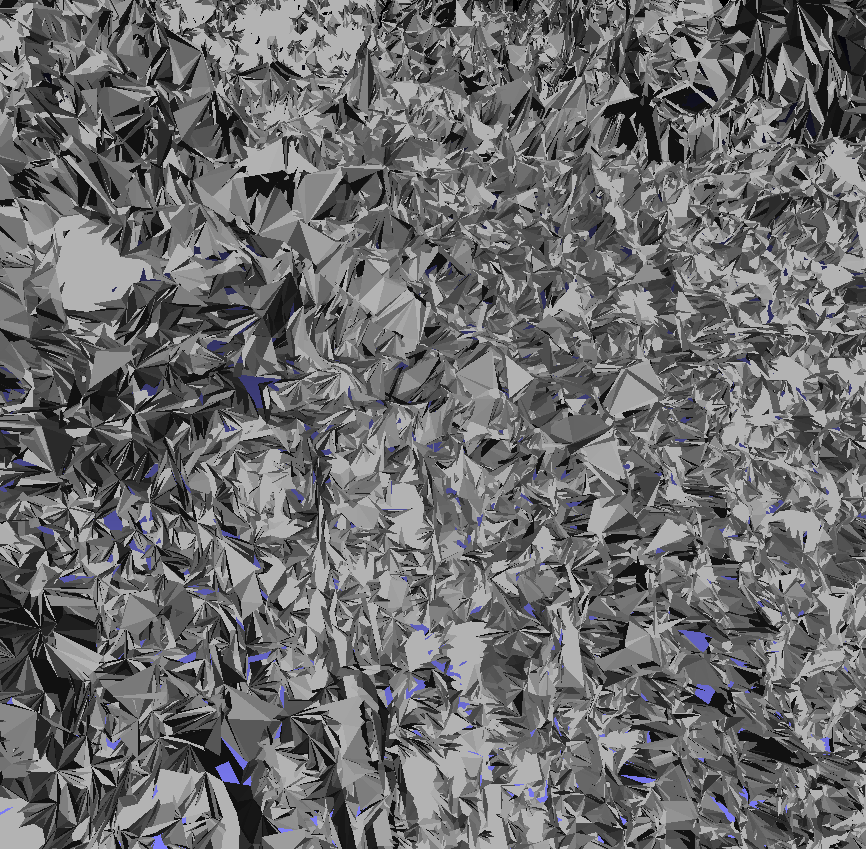
\includegraphics[width=180pt]{figs/greedy_closeup.png}
	\caption{Közeli kép a felületről \label{fig:greedy_closeup}}
\end{figure}

A meredekséget csökkenteni (de ezzel rontani az összekötöttséget) különböző szögek paramétereivel lehet, de nem érdemes, a felület simítására van szükség.

\subsubsection{Pontfelhő simítása}

Első ötletként a pontfelhőt ritkítjuk. Itt választhatnánk azt a megközelítést, hogy például minden $n$. sorból csak minden $n$. pontot választjuk, így lényegében $n^2$-tel leosztjuk a pontok számát, ez a viselkedés megfelel az előzőekben látott \texttt{OrganizedFastMesh} algoritmussal az oldalhosszt $n$-re állítva.

\begin{figure}[tbh]
	\centering
	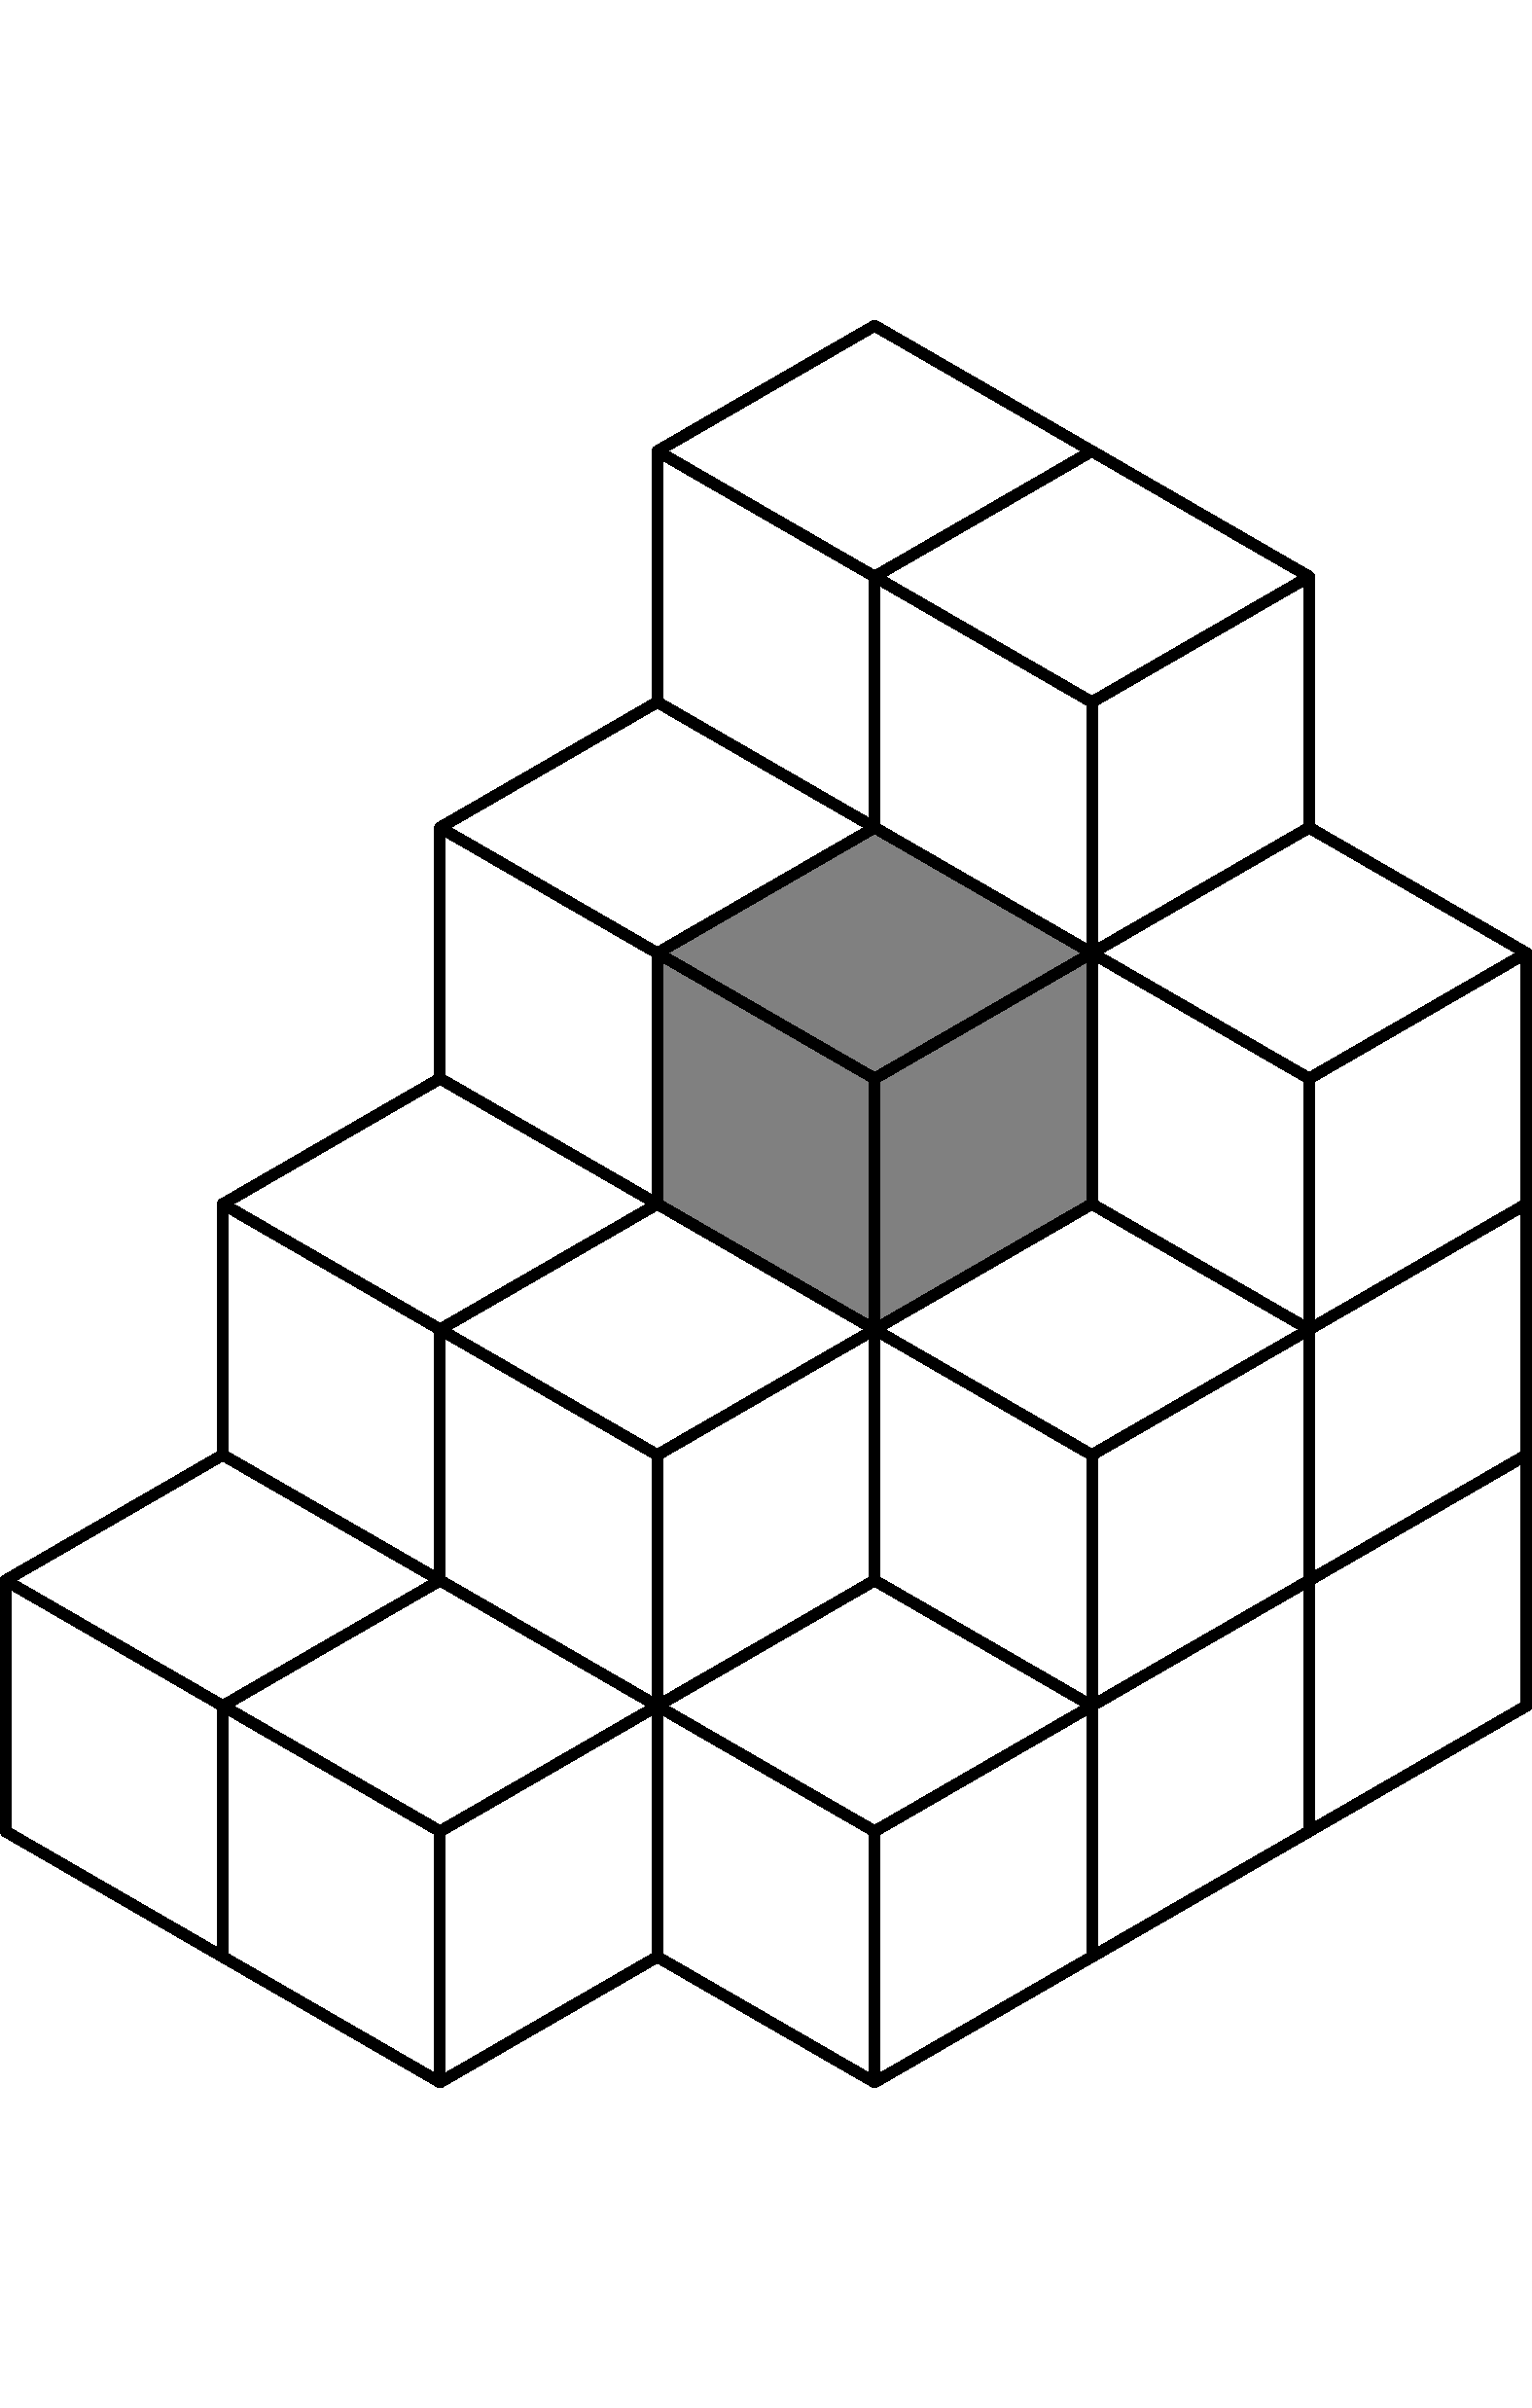
\includegraphics[trim=0cm 6.5cm 0cm 6.5cm,width=80pt]{figs/voxels.pdf}
	\caption{Voxel-háló kockákból \label{fig:voxel_grid}}
\end{figure}

PCL-ben lehetőségünk van voxel-háló (lásd \ref{fig:voxel_grid}. ábra) alapú ritkításra, melynek lényege, hogy megadott oldalhosszúságú téglatesteket illeszt egymás mellé, és az egy téglatestbe eső vertexeket az ő centroidjukkal helyettesíti. Ezzel pedig nem csak azt érjük el, hogy a pontok száma csökken, hanem simul is.

A 3D rekonstrukciós algoritmus a mélység értékeket nem találja el elég pontosan, így, hogy a $z$ tengely mentén simítsunk, olyan téglatestet választunk a háló építőegységeként, ami ,,mélyebb'', tehát $z$ irányban hosszabb, mint $x$ és $y$.

A ritkítás után már nem használhatjuk az \texttt{OrganizedFastMesh} algoritmust, mert elveszik a rendezettség, ezért a simított pontfelhőre az előzőekben szintén ismertetett \texttt{GreedyProjectionTriangulation} algoritmust használjuk ($\mu=2.5$ és 100 szomszéd vizsgálata) és így a simítás eredménye \aref{fig:voxelgrid}. ábrán látható.

\begin{figure}[tbh]
  \centering
  \begin{subfigure}[b]{.32\linewidth}
	\centering
	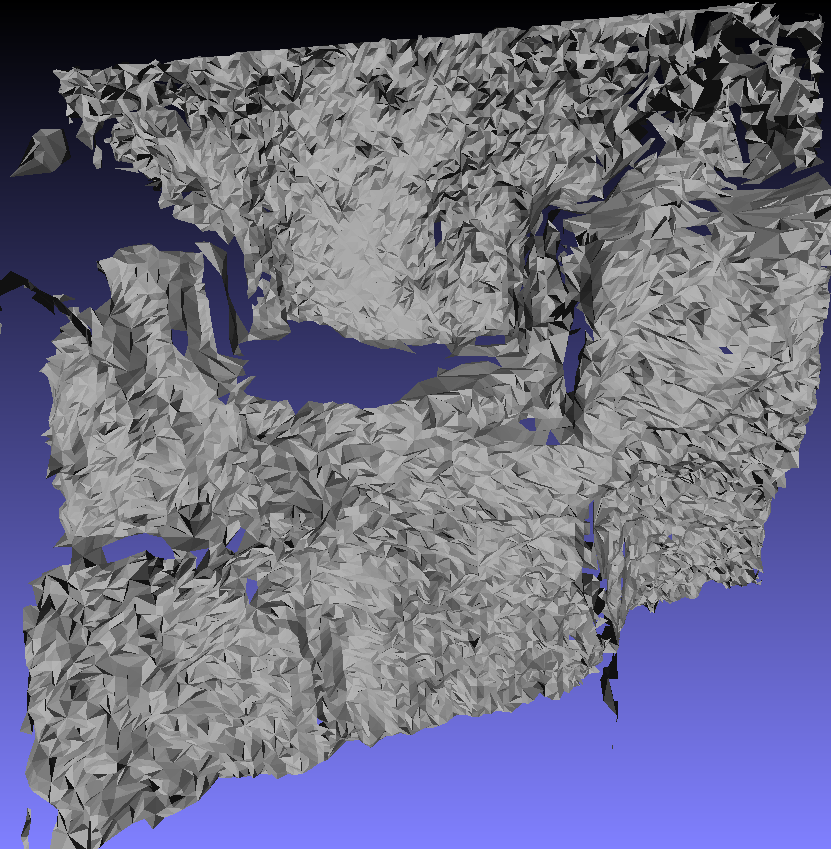
\includegraphics[width=100pt]{figs/voxel1.png}
	\caption{$0.05\times 0.05\times 1.0$\label{fig:voxel1}}
  \end{subfigure}%
  \begin{subfigure}[b]{.32\linewidth}
	\centering
	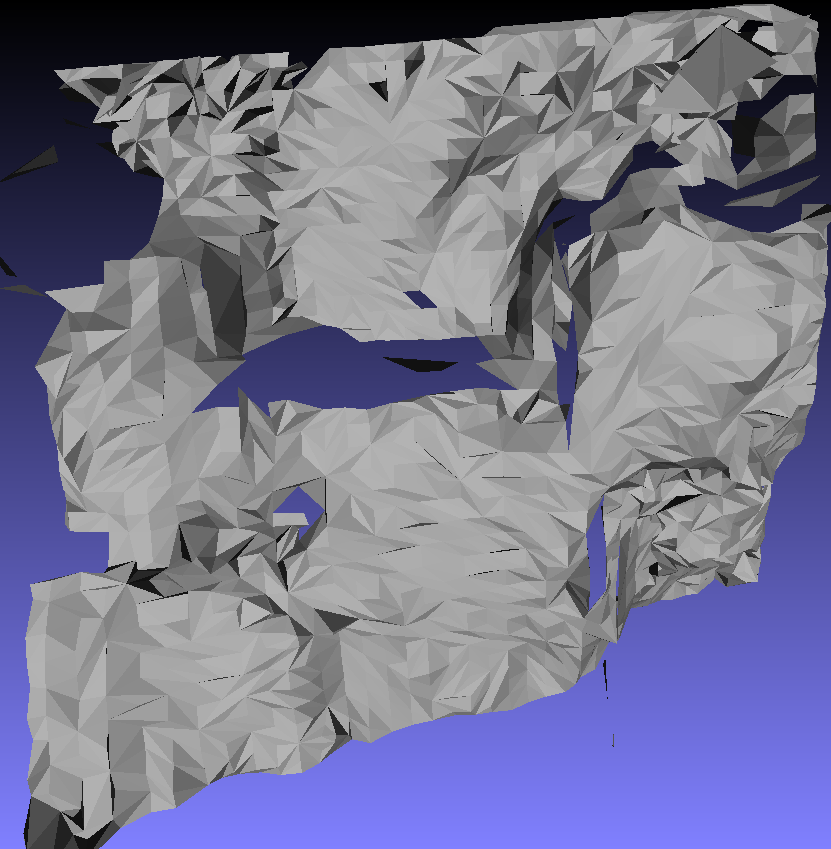
\includegraphics[width=100pt]{figs/voxel3.png}
	\caption{$0.15\times 0.15\times 1.0$\label{fig:voxel3}}
  \end{subfigure}%
  \begin{subfigure}[b]{.32\linewidth}
	\centering
	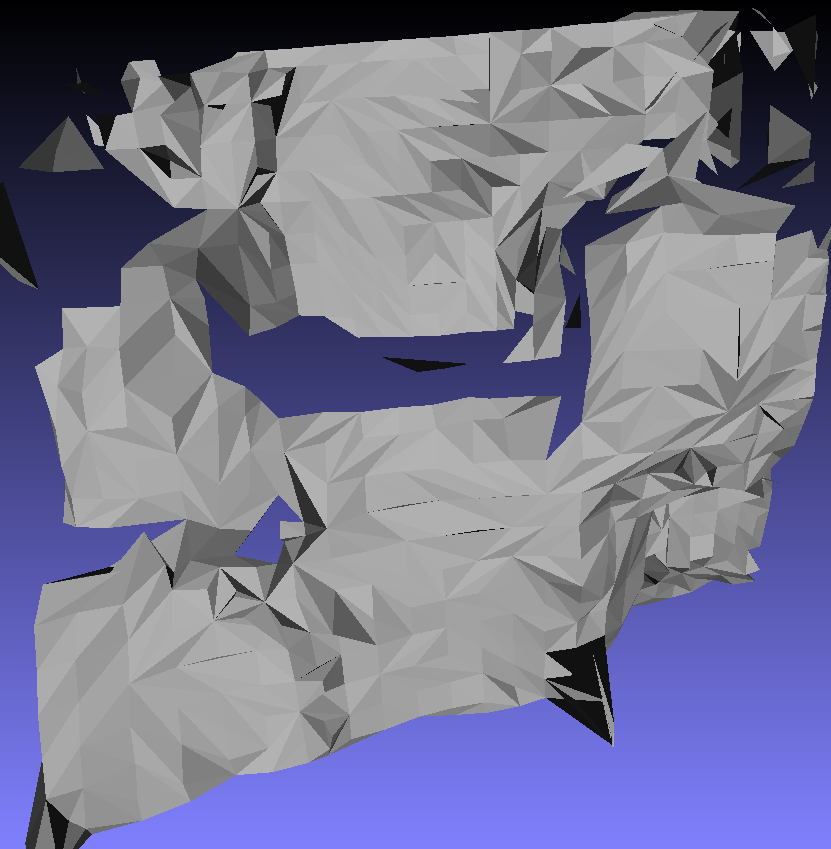
\includegraphics[width=100pt]{figs/voxel5.png}
	\caption{$0.25\times 0.25\times 1.0$\label{fig:voxel5}}
  \end{subfigure}%
\caption{Voxel-háló alapú simítás, különböző méretű voxelekkel \label{fig:voxelgrid}}
\end{figure}

\subsubsection{Pontfelhő sűrítése}

Megfigyelhetőek kiugró és különálló részek, pl. a balfelső sarokban a növény levelei, vagy a szekrény szélén lefutó kábel. Ezeket kisebb voxelekkel se tudjuk simábbá tenni (lásd \ref{fig:voxel1}. és \ref{fig:voxel3}. ábra), pusztán a háromszögek lesznek sűrűbben, de a felület töredezett marad. Viszont, ha a riktított pontfelhőben közbenső pontokat interpolálunk, akkor már részletesebb, de simább felületet kaphatunk.

Az általam használt módszer a ,,mozgó legkisebb négyzetek'' (\textit{Moving Least Squares -- MLS}) \cite{mls}, melynek található egy implementációja a PCL-ben is. A tényleges sűrítéshez szükség van arra, hogy a pontokra illesztendő függvényeket/felületeket hogyan nyerjük. Ezek közül kettőt vizsgáltam meg: \texttt{SAMPLE\_LOCAL\_PLANE} és \texttt{VOXEL\_GRID\_DILATION}. Előbbi a pontokra próbál illeszteni polinomális függvényeket (melyeket a szomszédok alapján számol), és ennek mentén a függvényeket érintő síkokon vesz fel négyzetrács-csúcspontokat. Ezt demonstrálja \aref{fig:upsampling-plane}. ábra.

\begin{figure}[tbh]
  \centering
  \begin{subfigure}[b]{.32\linewidth}
	\centering
	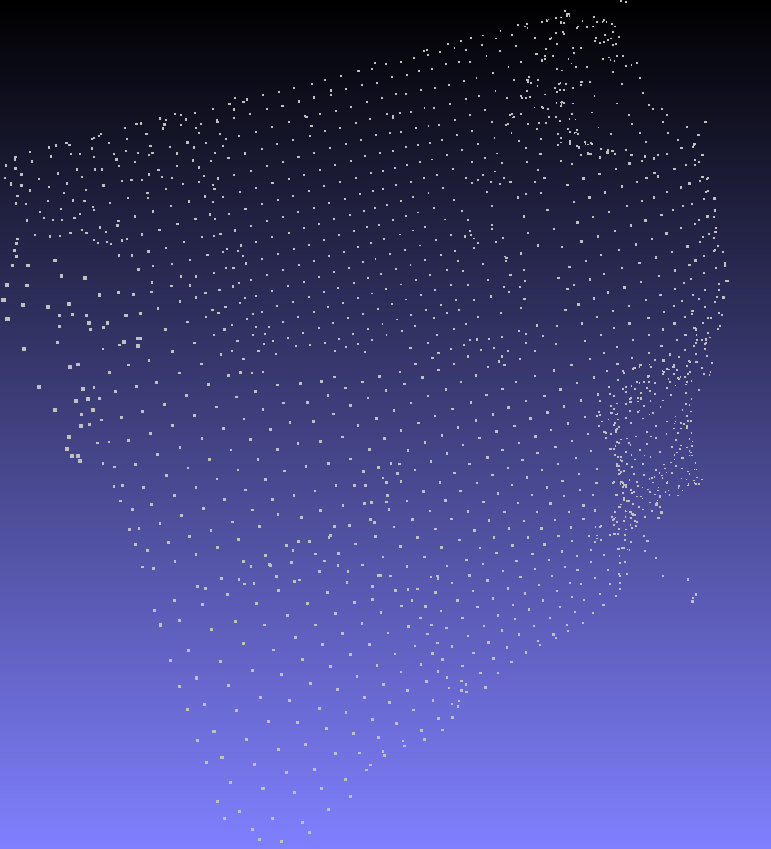
\includegraphics[width=100pt]{figs/plane00.png}
	\caption{ritkított \label{fig:upsampling-plane1}}
  \end{subfigure}%
  \begin{subfigure}[b]{.32\linewidth}
	\centering
	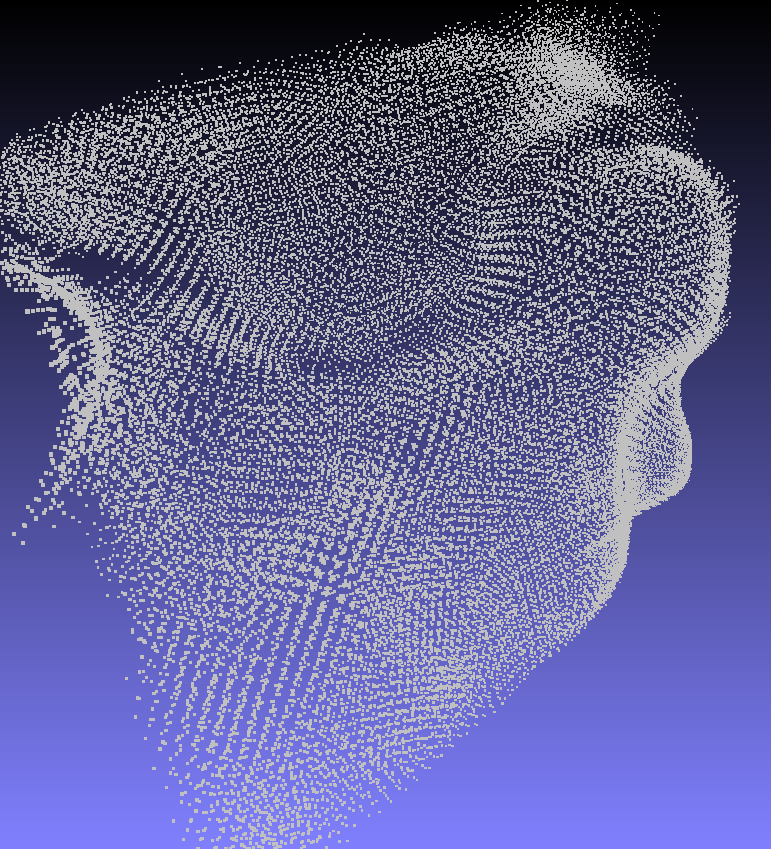
\includegraphics[width=100pt]{figs/plane01.png}
	\caption{sűrített \label{fig:upsampling-plane2}}
  \end{subfigure}%
  \begin{subfigure}[b]{.32\linewidth}
	\centering
	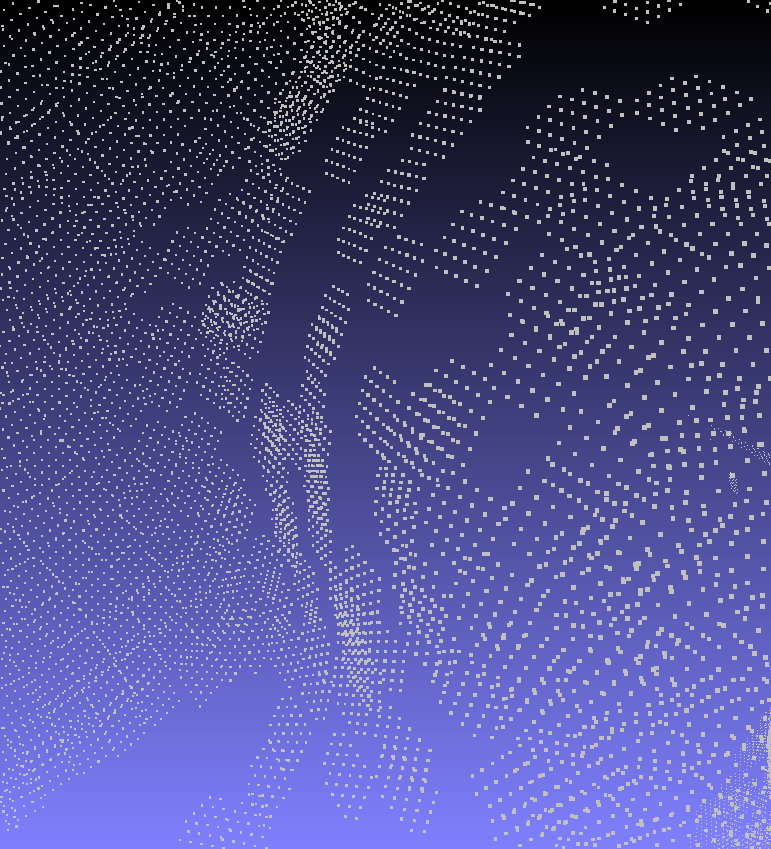
\includegraphics[width=100pt]{figs/plane02.png}
	\caption{közeli, torzítva \label{fig:upsampling-plane3}}
  \end{subfigure}%
\caption{\texttt{SAMPLE\_LOCAL\_PLANE} sűrítő módszer. Az első két ábra mutatja a változást, utóbbi pedig azt demonstrálja, hogy eltorzított paraméterekkel jól látható a síkok és az azokon lévő négyzetrács-pontok. \label{fig:upsampling-plane}}
\end{figure}

Utóbbi pedig a már jól ismert voxel-hálót alkalmazza: a pontfelhőt beteszi egy voxel-hálóba, majd a pontokra illeszthető polinomiális függvények (a pont környezetében) és a háló metszéspontjait nézi: amely voxeleken áthaladnak, azokat feltölti ponttal. Ezt \aref{fig:upsampling-voxel}. ábra mutatja be.

\begin{figure}[tbh]
  \centering
  \begin{subfigure}[b]{.32\linewidth}
	\centering
	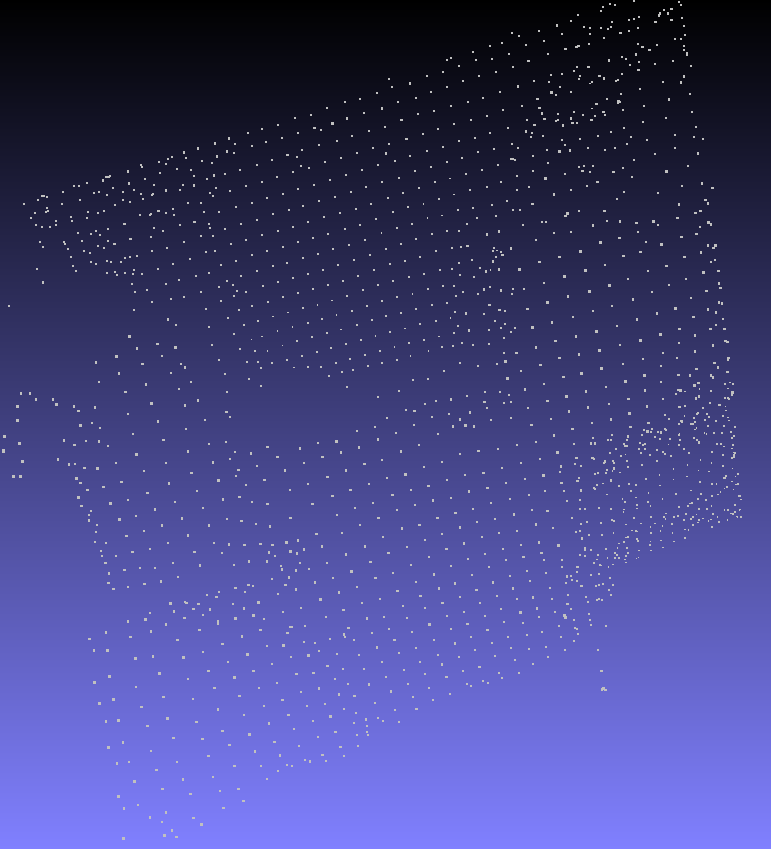
\includegraphics[width=100pt]{figs/voxel_up01.png}
	\caption{ritkított \label{fig:upsampling-voxel1}}
  \end{subfigure}%
  \begin{subfigure}[b]{.32\linewidth}
	\centering
	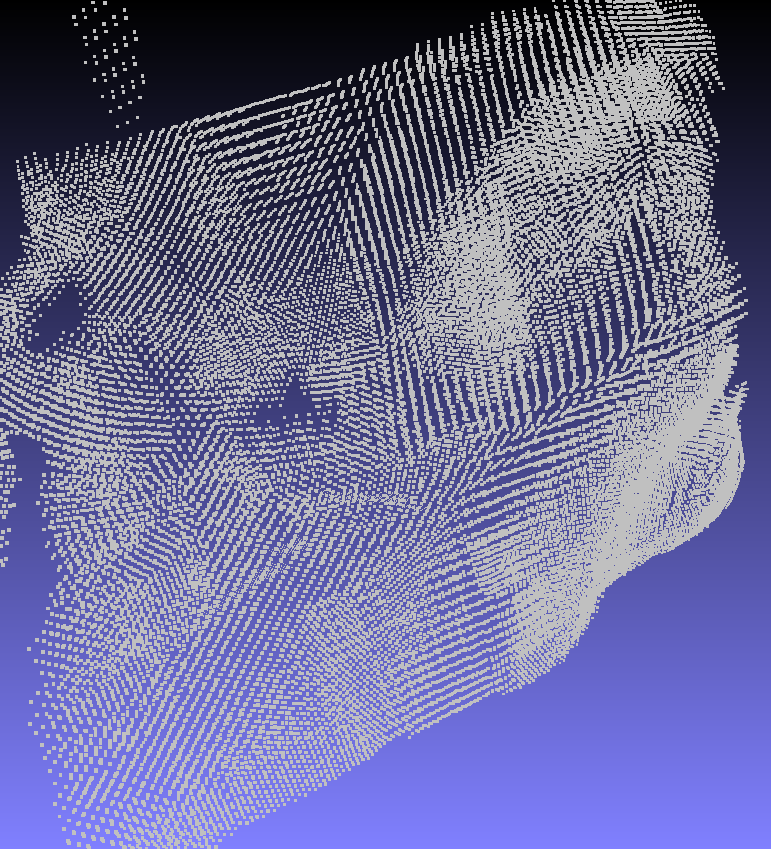
\includegraphics[width=100pt]{figs/voxel_up02.png}
	\caption{sűrített \label{fig:upsampling-voxel2}}
  \end{subfigure}%
  \begin{subfigure}[b]{.32\linewidth}
	\centering
	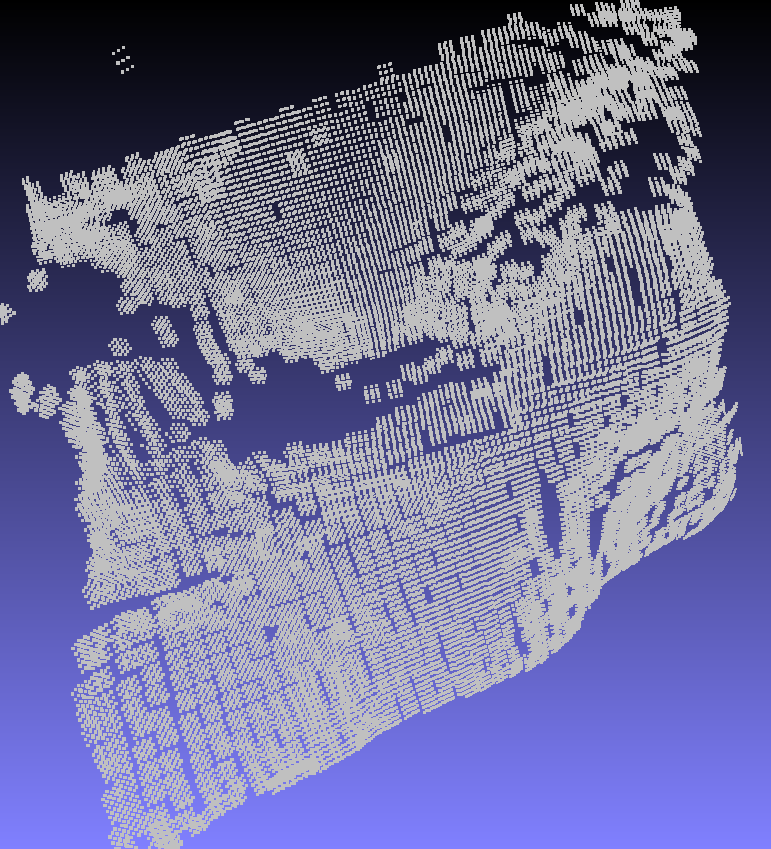
\includegraphics[width=100pt]{figs/voxel_up03.png}
	\caption{torzított paraméterek \label{fig:upsampling-voxel3}}
  \end{subfigure}%
\caption{\texttt{VOXEL\_GRID\_DILATION} sűrítő módszer. Az első két ábra mutatja a változást, utóbbi pedig azt demonstrálja, hogy eltorzított paraméterekkel jól látható a voxel-hálóból fakadó rácshatás (ebben a tekintetben küllemre hasonlít az előbbire). \label{fig:upsampling-voxel}}
\end{figure}

Ami érdekes, hogy ez az eredeti pontoktól távol is ,,talál'' pontokat és ott is sűríti ezeket, ezt célszerű lenne kivizsgálni későbbiekben, vagy statisztikai módszerekkel ezeket a távol eső pontokat kiszűrni.

Ezeket a sűrített pontokat megint ritkítva (már kocka-hálót használva), már egészen sima felületeket kapunk, talán túlzóan is. Álljon ennek bemutatásaként \aref{fig:final-surfaces}. ábra, a megfelelő paraméterek helyes megválasztásának meghatározása is az eljövendő félévek egyik feladata lesz. Megfigyelhetjük hogy a voxel-háló alapú jobban kitölti a hézagokat.

\begin{figure}[tbh]
  \centering
  \begin{subfigure}[b]{.49\linewidth}
	\centering
	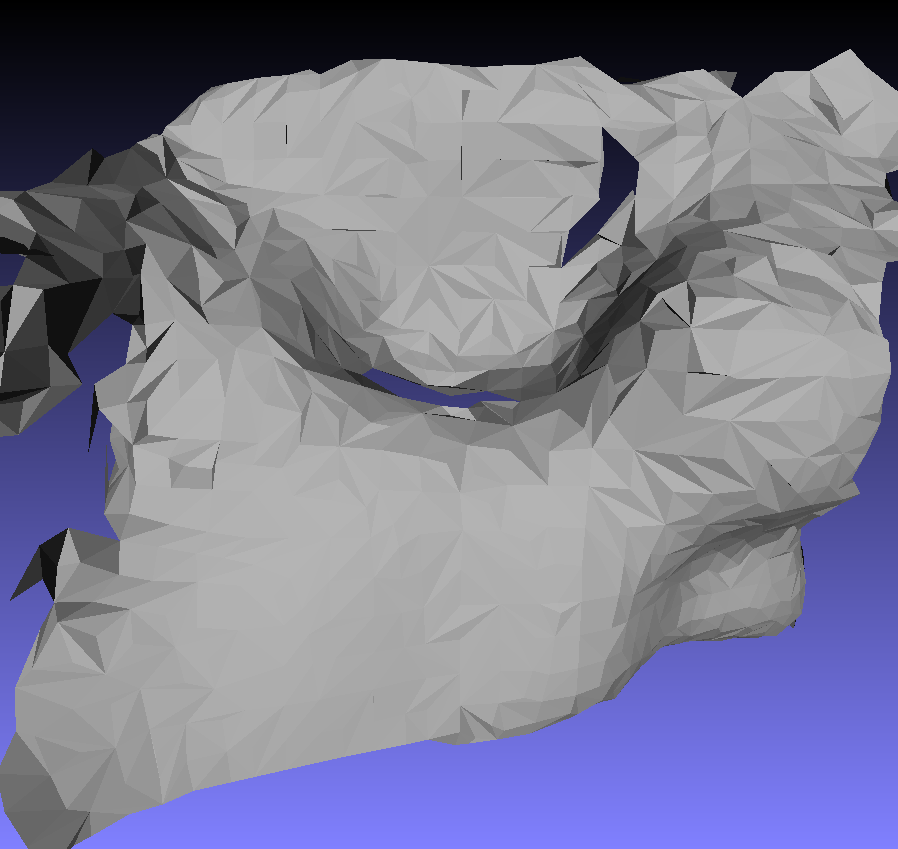
\includegraphics[width=160pt]{figs/final00.png}
	\caption{\texttt{SAMPLE\_LOCAL\_PLANE} \label{fig:final1}}
  \end{subfigure}%
  \begin{subfigure}[b]{.49\linewidth}
	\centering
	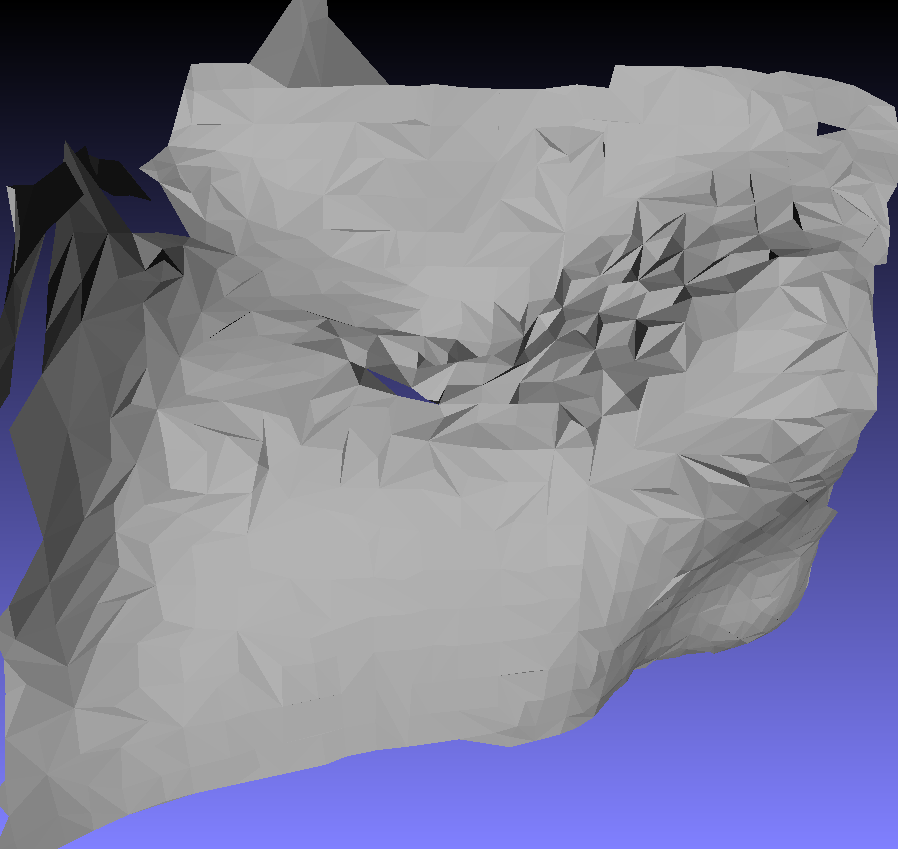
\includegraphics[width=160pt]{figs/final01.png}
	\caption{\texttt{VOXEL\_GRID\_DILATION} \label{fig:final2}}
  \end{subfigure}%
\caption{A két eljárás ritkítás és mesh-számolás után \label{fig:final-surfaces}}
\end{figure}

\subsection{Textúra vetítése}

\begin{figure}[tbh]
  \centering
	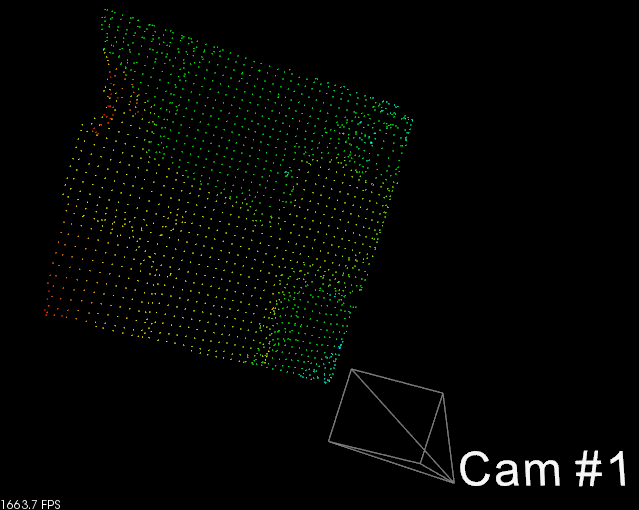
\includegraphics[width=150pt]{figs/projection.png}
	\caption{Textúra vetítése \label{fig:projection}}
\end{figure}

A PCL-ben rendelkezésre áll minden algoritmus ahhoz, hogy egy adott paraméterekkel rendelkező kamera által látott képet rávetítsünk egy \textit{mesh}re, de erről dokumentáció nem található, így szükség volt egy kis próbálkozásra, forráskód beható vizsgálatára. A kamera képét és felhasználva a kalibráció során nyert paramétereket sikeres volt a vetítés \aref{fig:final2}. ábrán látható hálóra, melynek eredménye \aref{fig:texture}. ábrán látható.

\begin{figure}[tbh]
  \centering
  \begin{subfigure}[b]{.32\linewidth}
	\centering
	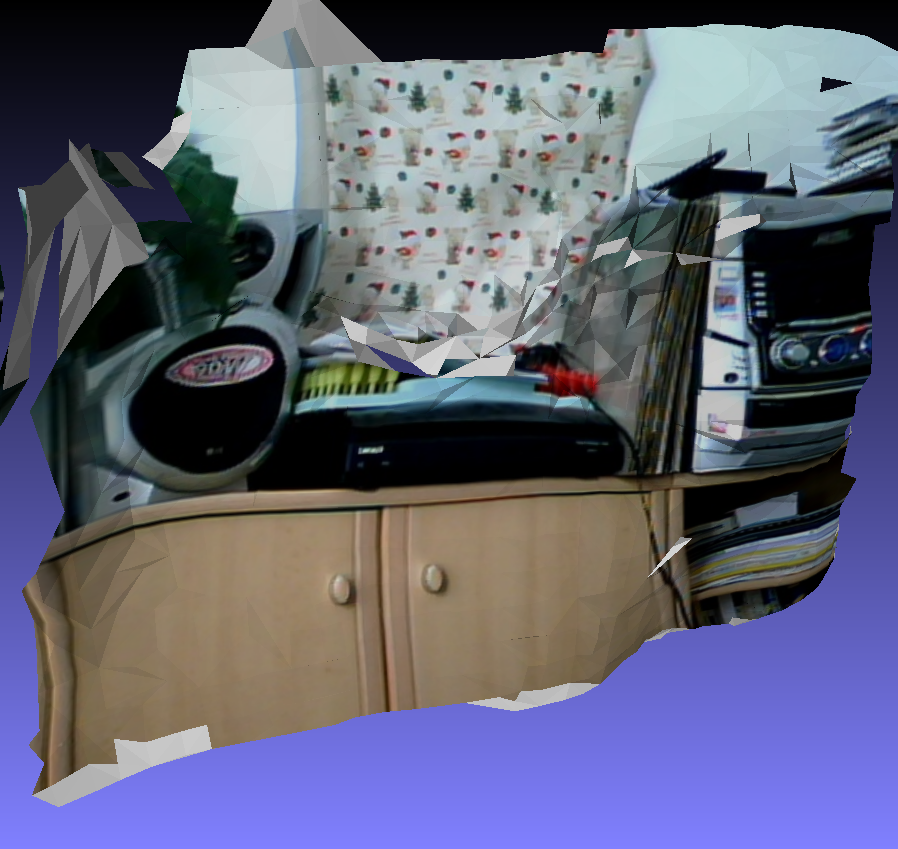
\includegraphics[width=100pt]{figs/texture00.png}
	\caption{szemből \label{fig:texture1}}
  \end{subfigure}%
  \begin{subfigure}[b]{.32\linewidth}
	\centering
	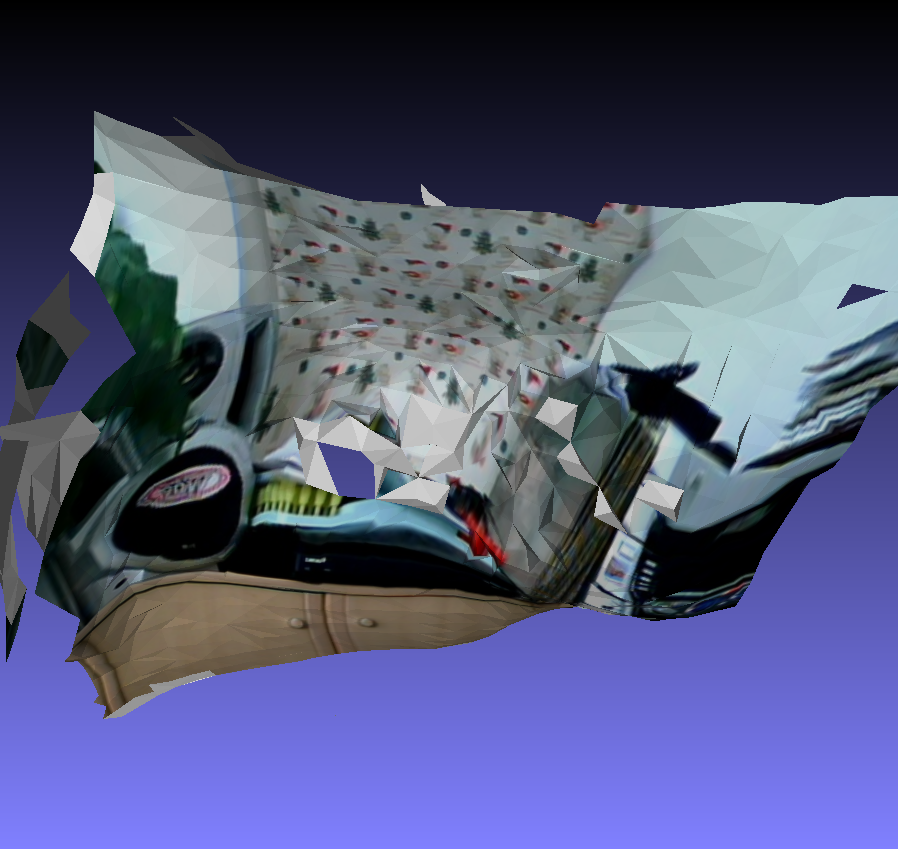
\includegraphics[width=100pt]{figs/texture01.png}
	\caption{felülről \label{fig:texture2}}
  \end{subfigure}%
  \begin{subfigure}[b]{.32\linewidth}
	\centering
	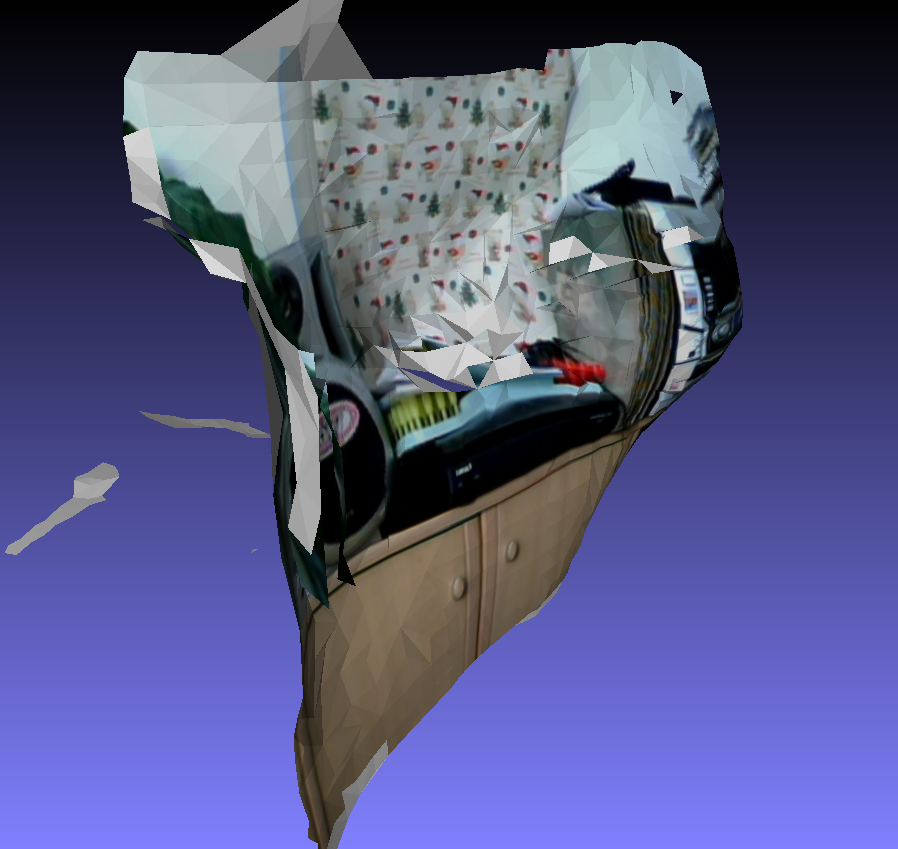
\includegraphics[width=100pt]{figs/texture02.png}
	\caption{balról \label{fig:texture3}}
  \end{subfigure}%
\caption{Textúrázott felület \label{fig:texture}}
\end{figure}

\subsection{Jövőbeni feladatok}

Könnyű meggondolni, hogy a fentiekben ismertetett lépések sztereovideóra (sztereóképek egymás utáni szekvenciája) is alkalmazhatóak. Érdemes azt is szem előtt tartani, hogy a térrészek statikus részeit (bútorzat, álló tereptárgyak) elég egyszer modellezni, és csak a mozgó objektumokat képkockáról képkockára modellezni (melyeket pl. a mélységinformációk felhasználásával úgy kaphatjuk, hogy ,,kivonjuk'' a hátteret a képből).

Izgalmas feladat még a több nézőpontból felépíthető pontfelhők, egy koordináta-rendszerbe történő transzformálása, így a térrész nagyobb részét tudjuk lefedni. Ezen lehetőségek vizsgálata a következő félév feladata lesz.

\subsection{Összefoglalás}
\label{sec:osszefoglalas}

A félév során elért eredmények összefoglalva:
\begin{itemize}
\item Elolvastam számos API dokumentációt, valamint a témához kapcsolódó online anyagot, publikációt:
\begin{itemize}
\item 3D rekonstrukció
\item felület (re)konstrukció
\item pontfelhők ritkítása és sűrítése
\end{itemize}
\item Megismertem a PCL alkalmazáskönyvtár bizonyos, a fentiekhez kapcsolódó részeit
\item Készítettem körülbelül 3000 sor C++-kódot
\end{itemize}

\newpage
 
%==================================================================
\section{Irodalom, és csatlakozó dokumentumok jegyzéke}
\label{sec:irod-es-csatl}

\printbibliography[title={Irodalomjegyzék}]

%==================================================================
\subsection{A csatlakozó dokumentumok jegyzéke}
\label{sec:csat-irod}

Az elkészült programkód, illetve a felhasznált fájlok az alábbi GIT repóban érhető el, melyből publikus klón készíthető:
\begin{center}
\url{https://github.com/messo/msc_onlab2}
\end{center}

A tárolóban a forrásfájlok és fejlécek találhatóak, valamint CMake segítségével Makefileok generálhatóak, amelyekkel különféle platformokon lefordíthatóak a futtatható állományok -- feltéve, hogy a legfrissebb PCL és OpenCV függvénykönyvtár rendelkezésre áll.

\end{document} 
